\subsection{Project Requirements}
\noindent The main purpose of the project is to create a file synchronizer that requires a central server to host the client and synchronize files, handle multiple simultaneous user requests, and handle conflicts. The requirement for this project is to ensure that the server can handle multiple simultaneous clients and conflicts with the same copy of the file, so we must have at least two clients and allow different types of users to upload files to the server. First, we need to design a desktop, which can be a command line or a background utility. In addition, we need a mobile client, which is a standalone application developed in the iOS or Android environment.




\begin{comment}
\noindent As our main task is to develop a multi-host file synchroniser, in summary, the function of this synchronizer is to make it possible to edit the same files across multiple computers in a sensible way. This synchroniser can satisfy the multiple clients access and edit the data in a single central server. In this group project, our final result is to develop a server and two clients, one for desktop and another for mobile.the function of this synchronizer is to make it possible to edit the same files across multiple computers in a sensible way. This synchroniser can satisfy the multiple clients access and edit the data in a single central server. In this group project, our final result is to develop a server and two clients, one for desktop and another for mobile.
\end{comment}



\subsection{Project Design}
\noindent Our project design is based on the project's requirements. After the unanimous consent of all the team members, we have come up with many ideas and modifications. It will be described in detail how we designed this synchronization project from the following points:

%\noindent The desktop client team decided to develop a web application for the user to easily upload and download files from the server using the UI instead of using the command line.
%The mobile client team has decided to implement in the iOS environment because members have previously developed experience with the application in this environment.
\subsubsection{Server Design}
\noindent Now the mainstream web server software is mainly composed of IIS, Tomcat or Apache. IIS supports ASP and can only run on Windows platform. Apache and Tomcat are roughly the same, but Apache supports static pages as Tomcat supports dynamics pages, such as servlet class. If you use the Apache and Tomcat together to develop servers, in this scenario, Apache is only used as a forwarding intermediate processor, the processing of JSP is handled by Tomcat. Both Apache and Tomcat support PHP, CGI, JSP and can run on multiple platforms and they are the world's top level web server platform. Although Windows is easier to use, considering that our front end client wants to use ThinkPHP, we finally chose the Apache and Tomcat.

\subsubsection{LAN Interaction Design}
\noindent We initially thought about putting data into the cloud, so that we can achieve synchronous uploading and other functions under different network platforms. However, we need to rent a server and take into account the cost of test development, we finally put it in the LAN. This avoid network transmission problems and are more convenient to collaborate on development.

\subsubsection{Preliminary Design of the Database}
\noindent First, we identified several basic features we needed and customized the sketches. The most basic feature we want to solve is that multiple users upload and edit files at the same time. For this purpose we first need a user table for storing the user's UID and name, password, etc. Secondly we need a file table for storing file IDs, file names, creators, etc. Next, set up a authority table for viewing file permissions. Here, the file ID is used as the primary key. In consideration of possible problems during the operation of the program, in order to better understand our project, we also designed an error log table for the synchronization error occurred in the upload operation for checking.

\vspace{0.3cm}
\noindent This is just a preliminary design and based on this design, we started to write the code of the database part as well as write the basic forms in the database. With the implementation and requirements of the later functions, we will modify the entities and entries of the database according to the specific situation.

\subsubsection{File Upload Conflict}
\noindent After group discussion, our solution is that when the system determines that two users have performed the download operation, we will first mark the version of the document, and the version will be automatically added when uploading. When the uploading detects that the existing version of the database is greater than or equal to the uploaded version, a conflict is found. The second uploader is told and asked that another user edits the file while he is editing. The second uploader then selects the version and then overwrites the database version. The uploader and upload time will be recorded in the version. The next user will see all historical versions when searching for this file and can open or choose to download them.


\subsubsection{The Final ER\_design for Database}
\begin{figure}[H]
  \centering
  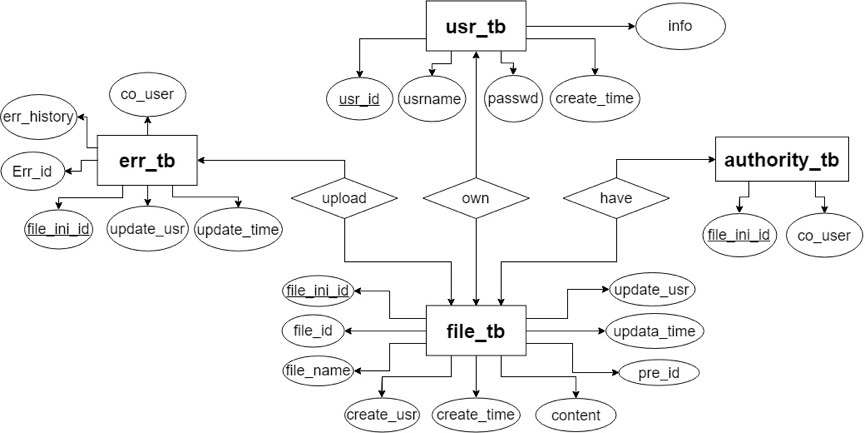
\includegraphics[width=.8\textwidth]{designdb.png} %图片文件的相对路径
  
  \label{png0} %此处的label相当于一个图片的专属标志,目的是方便上下文的引用
\end{figure}

\subsubsection{Transmission Protocol Design}
\noindent When choosing HTTP and HTTPS protocols, we originally wanted to choose HTTPS protocol. HTTPS protocol is a network protocol built by SSL+HTTP protocol for encrypted transmission and identity authentication. It is better than http protocol security and can better protect users’privacy. But considering that https needs to apply for a certificate, and there are very few free certificates. Finally, we still chose the HTTP protocol, which is relatively simple and convenient.

\subsubsection{UI Design}
\noindent After designing the first draft of the database, we have roughly identified some of the function keys for our UI interface design. The first is the welcome screen, there will be two options for registration and login. After logging in, you will be taken to the user's main page. You can see the user documentation and user information, in this page user can also upload and create new files. Click to enter the file page, the user can edit and rename the text, and the user can also add or delete the permissions of other users to this file. When there is a conflict in the uploaded file, there will be a file comparison page for the user to select the file they want to save.

\subsubsection{Some Other Details}
\noindent After completing the login screen, we first added the registration feature to join the new user. After the file modification function is completed, we have added the file renaming function for the file name that may need to be modified. Since we have considered that the file sync upload may overwrite the previous user's article, or if the user wants to view the old version and edit it, we have added the history section to view the old version. On this basis, we have adjusted the database again.

